\section{Analysis}\label{sec-análise}

In this section, we will analyze the 21 articles selected for the systematic literature review on the concept of AL. All of the analyzed articles are detailed in a table in Annex I, which includes the name of the authors, year of publication, title of the article, type, and place of publication. We will first present an analysis of the publications' metadata, including the year of publication, authors, journals, or events in which they were presented, along with other relevant details. Next, we will effectively analyze the corpus, considering the questions that drive our investigation.

\subsection{Initial perspectives from metadata}

When analyzing the list of publications, we observed that the data covers a period of four years, from 2019 to 2022 \Cref{image-02}. Notably, most publications are concentrated in the years 2021 and 2022, in which 6 and 10 publications, respectively, were found. This concentration of debate on the concept of AL over the past four years, as well as the upward trend in the number of publications on the topic, may indicate increased recognition of the importance of understanding algorithms and their roles in contemporary social life, as well as the advancement of discussions surrounding AL.

\begin{figure}[!h]
\centering
\begin{minipage}{0.85\linewidth}
\caption{Number of publications per year.}
\label{image-02}
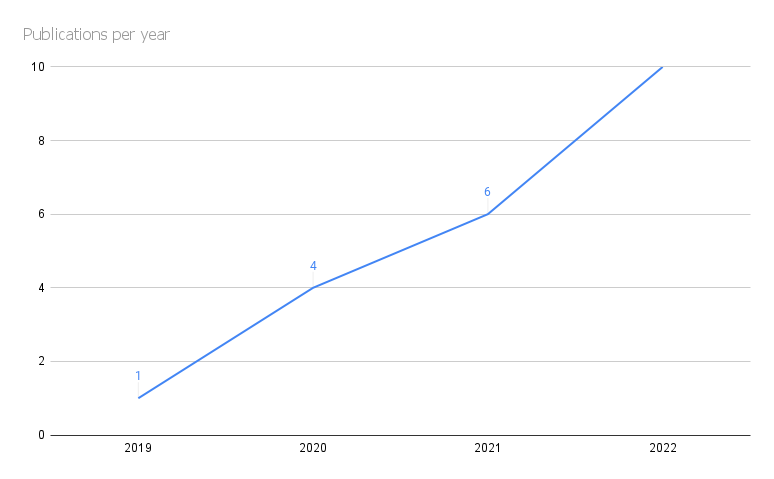
\includegraphics[width=\linewidth]{image2_en.png}
\source{Created by the authors.}
\end{minipage}
\end{figure}

Regarding the origin of the publications, it is possible to observe a diversity of formats, covering articles in periodicals (15), book chapters (2), and articles in the annals of academic events (4). As seen in the table in \Cref{anexo-1}, only two journals contain more than one article on the topic (AI and Society and Computers and Composition). It is noted that the studies found cover a wide range of areas: communication, computing, psychology, information science, education, in addition to other disciplines related to the debate on information and communication technologies (such as Human-Computer Interaction). This aspect may indicate the multidisciplinary interest in the topic and the relevance of the notion of AL in different academic contexts.

At this stage of the analysis, the absence of texts in Portuguese and the low number of publications in Spanish were also noticed among the 21 articles selected for the systematic review on AL. This observation may indicate a scenario of scarcity of investigations on the topic in the Latin and Ibero-American context.

With this information as a basis, the next stage of our analysis provides a more in-depth study of these publications, considering the guiding questions of the investigation on conceptual proposals, pedagogical techniques, practical applications, and difficulties related to AL.

\subsection{Exploring the foundations of Algorithmic Literacy (AL): conceptual models, distinctions, and multidisciplinary applications}

The analysis of articles that address AL reveals a diverse and complex scenario, in which no conceptual unity is observed. It was first noted that the debate surrounding AL has proposals that derive from pre-existing and more consolidated literacy approaches, such as information literacy, literacy for the digital environment, and data literacy \cite{Lloyd2019}. These approaches emphasize the process of creating individual awareness on how information is produced, classified, and distributed in different environments \cite{Bakke2020}. In these studies, AL emerges as a response to the effects of the introduction of algorithmic agency, a series of more specific skills in the scenario of a datafied life \cite{Kampa2021}. In this context, calls for literacies are often a response to new technologies that create new power structures \cite{Devito2021}.

For \textcite[p. 3]{Ridley2021}, AL is one of the offshoots of the varied literacies of the digitalized world: “Although each of them has its own domain and focus, they share common ideas and are generally symbiotic with each other”. Similarly, \textcite[p. 30]{Devito2021} argues that AL should not be observed in isolation, but rather as “a component of a broader platform literacy that encompasses all of the literacies mentioned previously”. For \textcite{Lloyd2019}, what differentiates AL from more general literacy proposals is that it requires an in-depth examination of the development culture of these systems, a movement that is in line with research proposals, such as that of \textcite{Seaver2017}. “According to this perspective, building an algorithm is a practice that is embedded within other practices and is influenced by specific views of the world” \cite[p. 1483]{Lloyd2019}.

In this context, the specificity of AL in relation to other digital pedagogical approaches lies in the need for a critical examination of characteristic properties of algorithmic agency, based on notions such as performativity, opacity, diversity, trust, bias, and social justice \cite{Lloyd2019}. In addition, \textcite{Devito2021} indicates that any AL proposal must deal with the unstable nature of algorithmic systems in constant transformation, incorporating this flexibility and ability to update into pedagogical constructions. For the author, this makes it essential to recognize that “subjects are already immersed in the environment in question, making AL an exercise mainly to formalize and correct the knowledge found in the world, rather than introducing purely new knowledge” \cite[p. 3-4]{Devito2021}.

In the analyzed studies, one of the main goals for AL is the development of awareness concerning the agency of algorithmic systems in different interactions with subjects \cite{Bakke2020}, whether in the search for information and content \cite{Kampa2021}, in interaction with automated interaction systems \cite{Shin2022} or in relation to algorithmic personalization \cite{Devito2021,Lv2022,Bell2023}. According to \textcite{Ridley2021}, this is a way of recognizing and raising awareness about the forms of power of this technological standard and, at the same time, emphasizing the empowerment possible for subjects in the face of these structures. In this approach, LA can be defined as the ability to be aware of both the presence and developments of algorithmically driven systems and, thus, crystallize this understanding into a strategic use of these systems so that the subjects participating in this process can achieve individual or collective objectives \cite{Devito2021}. Therefore, AL should be understood as more than instructions for a more efficient use of algorithmic systems. It is an ideological practice of producing meaning and subjectivizations that are dissonant with what the performativity of these systems allows \cite{Ridley2021}.

In the next segment of this analysis item, two constituent dimensions of the debates that emerge from the examined articles will be explored. First, the meaning of the notion of critical empowerment will be discussed. After, the spectrum of different levels of awareness of subjects in relation to algorithmic systems will be addressed. Both debates are key to the conceptual AL proposals analyzed in our study.

\subsection{Critical empowerment: paths of agency in the face of algorithmic systems}\label{sub-sec-empoderamentocritico}

Power and control are two core notions in the debate established by the critical literature on algorithms. \textcite{Magalhaes2018} maintains that part of the literature, which he calls the damage paradigm, considers the power of algorithms as both a result and a driver of an original disparity between subjects (who have their lives affected by the analysis of digital data without being aware of it), and platform operators (who deliberately and strategically control the collection and analysis of this data). As \textcite{Rieder2018} indicates, these approaches are often geared towards simply denouncing the political and social effects of algorithmic systems, neglecting the analysis of how these infrastructures are articulated materially and discursively to produce the effects of power.

In analyzing the articles in the sample, it seems clear to us that power and control are issues for which the investigations analyzed seek to offer some type of answer or critical approach. In them, LA tends to be positioned as pedagogical knowledge for the development of critical consciousness and, consequently, the expansion of the subjects' agency capacity. It is in this context that the notion of critical empowerment emerges as an expected result of AL. In the conceptual proposals analyzed, there is an emphasis on individual empowerment based on the ability to critically observe the ways in which these systems function \cite{Bakke2020,Konig2022}.

\textcite{Konig2022}, for example, maintains that AL can form subjects with a reflective stance in relation to algorithmic systems, allowing them to understand that, with each suggestion or result generated by these systems, there are tractions of objectives, interests and assumptions that are not necessarily clear. Similarly, \textcite[p. 1483]{Lloyd2019} understands that reflection processes are central to literacies; thus, they can collaborate to generate attention on how “algorithms are expressed and operationalized (through our actions and interactions with interfaces and programs), along with the conditions, assumptions, and biases that are inherent in their production and operationalization”. \textcite[p. 177]{Sued2022} indicates that critical awareness and knowledge developed from AL can guarantee subjects “greater agency and freedom of action”.

However, warns \textcite{Konig2022}, critical empowerment as a result of AL proves to be limited for two reasons. First, the effect of a critical understanding of algorithms is naturally restricted, as there is no guarantee that people will be able to incorporate this knowledge and attitudes to exercise control over the operations of an algorithmic system. The configurations, interfaces, and rules of these systems often act to limit the possibilities for individual choice. Even if it is possible to grant users more control through individual influence over the configuration and behavior of the system, a second obstacle remains: the production of a more active and engaged stance of these subjects in the process of defining their objectives, interests, and values within these systems.

Therefore, in the debate about AL, the ability to develop a critical awareness in relation to algorithmic systems is seen as a way to expand the subjects' agency, a critical response. In this sense, in accordance with \posscite{Siles2024} approach, we consider that the debate on AL is intertwined with the notion of agency. When looking at what people do with algorithms, \textcite{Siles2024} proposes a more fluid agency approach, which derives from the bricolage between discussions in Cultural Studies and Science and Technology Studies. In this proposal, the relationship with algorithms comes to be seen less as solid opposite poles or definitive states and more as relationships of convergence, instability, coexistence, friction, and change. Sometimes users follow the algorithms' suggestions, other times they resist them. Often, they have both positions in the same actions. It is now considered that agency is a relational process that takes place in the intermediate space of the relationship between subjects and algorithms \cite{Siles2024}.

In the next item, reflections on the different levels of awareness about the functioning of algorithmic systems are discussed, a prominent point in the literature on the topic.

\subsection{Levels of awareness and perception about algorithms}

Awareness about the existence and functioning of algorithms is a recurring theme in discussions about digital platforms. Initial research, carried out in the middle of the previous decade, indicated a low level of awareness about the existence and functioning of algorithms \cite{Eslami2015}. \textcite{Bucher2019}, for example, investigated the way people become aware of algorithmic agency, suggesting that the imagination about the functioning of these systems can condition the way these individuals develop their practices on a given platform.

In the debates observed in our study, the subjects' perception of algorithms is positioned as a central factor in AL, based on the premise that the ways of understanding these systems can significantly shape the subjects' practices and interactions with their digital environments. In the studies observed in the analyzed sample, different approaches can be noted that dialogue with this issue. \textcite{Bell2023} point out that awareness about the functioning of algorithmic systems can vary dramatically in a similar group. In the study, it is indicated that the perception about algorithmic systems can vary between platforms and is usually more verbalized when talking about services in which personalization systems are more prominent in use, such as TikTok \cite{Bell2023}. According to the authors, this perception may even depend on the way the topic is presented to the subjects (for example, based on the variation in terms chosen, such as algorithm or personalization). Findings from \textcite{Lv2022} correlate this awareness with teenagers' intention to resist algorithms on online platforms. For the authors, the different levels of awareness and knowledge about algorithms are related to the willingness of adolescents to search for ways to deal with or avoid these systems \cite{Lv2022}. The study by \textcite[p. 352]{Parnell2022}, which analyzes queries to online search engines, presents empirical findings that indicate that “greater algorithmic literacy has a positive effect on self-reported skills in using search systems and a more frequent use of the Internet”.

In these studies, it is possible to perceive an effort to create parameters that make it possible to measure degrees of awareness and knowledge about algorithmic systems. These would be degrees of AL that can be identified based on the subjects' practices. One of the proposals that most advances this purpose is that of \textcite{Devito2021}. The author seeks to establish categories to stratify these different levels of consciousness and knowledge, which she calls the Levels of Complexity of Individual Theorization. The degrees of understanding observed by the author are developed, mainly, from folk theories, or informal theorizations, as a result of the subjects’ experience in their relationships with algorithmic systems and, at the same time, from contact with other content that addresses the topic. Such content becomes incorporated into the ways in which these subjects organize their practices \cite{Devito2021}.

The stratification proposed by the author is divided into two levels that each have subdivisions: the first is Functional Theorists, which portrays subjects who have initial awareness and limited understanding of the functional aspects of algorithms. This category is divided into Basic Awareness (when the subject identifies that an algorithmic system is in operation on a platform, having some effect, but does not affirm or cannot reflect on what specific effect) and Causal Powers (when the subject indicates that an algorithmic system is the cause of a given result). The second level is that of Structural Theorists, which highlights subjects who make substantial adjustments to their tactics in order to deal directly with algorithmic issues, expanding their sources of information. This category is divided by \textcite{Devito2021} into Mechanistic Fragments (when the subject indicates that an algorithmic system plays specific roles on a platform and believes that it has identified multiple factors that are weighted by the system to make decisions) and Mechanistic Ordering (when the subject perceives that an algorithmic system plays specific roles on a platform and believes that it has identified not only multiple factors used to make decisions, but also the order in which these criteria are applied or the relative weight of each of them).

Therefore, subjects' perception and knowledge about algorithms emerge as crucial issues in the context of AL. The literature analyzed demonstrates that the understanding of these systems can vary significantly between the subjects and the platforms observed, a variation that can considerably influence their interactions and digital practices. Furthermore, empirical research suggests that higher levels of awareness about algorithms are related to a greater willingness to create more strategic ways of interacting with these systems. The categorization proposed by \textcite{Devito2021} to stratify different levels of awareness and knowledge about algorithms offers an interesting approach to evaluating and understanding these differences. However, it is necessary to highlight the contingent role that individual uses and practices can have in the context of the relationship with algorithms, as well as the aforementioned unstable nature of these systems. These factors make any generalizing proposal about levels of perception and knowledge limited.

\subsection{Pedagogical proposals in the context of algorithmic literacy}\label{sub-sec-aspropostaspedagogicas}

The analysis developed in our study made it possible to observe in the articles studied a set of pedagogical proposals developed with the aim of promoting knowledge and awareness about the performance of algorithmic systems. It is interesting to note that the proposals observed do not form a methodologically uniform set. There are different paths for the development of AL, which are presented below.

When trying to systematize the methodological paths of AL \textcite{Silva2022} indicate two possible paths. The first consists of building basic knowledge by exploring the objectives of the developers of these systems and the effects of these technologies on our societies. This approach, which we classify as content-based, is developed by offering solid information about the underlying purposes of algorithms and how they affect different dimensions of everyday life. The second path focuses on the production of experience through interaction with algorithmic systems. In this case, learners are encouraged to explore the functionalities of the algorithms, seeking to develop their schemes and knowledge to explain how they work and how their decisions are made.

Exploring the experiences developed by subjects in contact with algorithmic systems is also a central pedagogical proposal of \posscite{Devito2021} study. As already highlighted, the author focuses her discussion on folk theories to “explain the results, effects, or consequences of technological systems” \cite[p. 4]{Devito2021}. This proposal is premised on the notion that we already have, to a greater or lesser extent, some experience with these systems, therefore AL should be primarily the exercise of formalizing and correcting knowledge found in the world, rather than purely introducing new knowledge \cite{Devito2021}. The methodological purpose of AL defended by \textcite{Devito2021} is to develop learning modes that lead subjects to a structural understanding of these systems. This involves both understanding that algorithms have an effect on specific outcomes and identifying the various specific factors that are weighted by the algorithms and the order in which these criteria are applied.

\textcite{Ridley2021} rely on the literature concerning computational thinking to develop pedagogical proposals in the field of AL. For the authors, these two notions have an interesting correlation and, therefore, the extensive literature on computational thinking is considered by them as fruitful for AL \cite{Ridley2021}. The authors consider that such an approach can help develop an understanding of algorithms and their processes, interpret their uses in different systems, and create and apply algorithmic techniques and tools to solve problems in a variety of domains.

On the path of pedagogical development based on experiences, \textcite{Klumbbyte2020} discuss the promotion of AL through pedagogical approaches that use critical design for interaction with algorithms. The authors' proposal centers on the idea of developing the Social Privilege Estimator, a social scoring system based on facial recognition and classification, which was built as a critical design artifact to raise awareness about existing inequalities and the adverse effects of security systems of facial recognition. Moreover, in the field of design, \textcite{Cech2020} proposes a debate on co-design measures to support the development of AL and the understanding of algorithmic processes. Through participatory and user-centered design principles, the author suggests the collaborative design of material and procedural solutions to understand algorithmic and promotional processes in these systems.

Finally, we observed proposals that establish what we call narrative interaction as a method for developing AL: pedagogical methodologies that are based on the development of experiences based on narrative proposals, such as games and dynamics, in which subjects are invited to act and make decisions as if they were developers of these systems. \textcite[p. 199]{Aleman2021} present the proposal for a digital game in which subjects are placed in interaction with “an engaging narrative and a programming environment that demonstrate the limitations of predictive models”. The authors' proposal seeks to lead educators and students to examine the biases of algorithmic models, thus  encouraging reflection on the tensions with algorithmic systems in their lives.

In a similar way, \textcite{Jeong2022} propose the implementation of educational initiatives, focusing on the YouTube recommendation system based on a dynamic that seeks to place elementary school students in the shoes of the algorithm, as responsible for defining what is relevant on the platform. The authors' proposal is inspired by the methodology developed by \textcite{Grosman2022}, which consists of a dynamic that offers participants data and objectives for making musical suggestions on YouTube. According to \textcite{Jeong2022}, the proposal aims to encourage young people to understand how recommendation algorithms work and affect their interactions with YouTube.

Still in the context of the classroom, \textcite{Koenig2020} proposes textual production in diaries as a pedagogical methodology to encourage students' reflections on their interactions with platforms. The author's proposal basically consists of creating individual diaries to explore and reflect on their own interactions with algorithmic systems. It encourages reflection on students’ experiences with platforms based on textual production about experiences and habits. From the empirical experiment conducted, \textcite{Koenig2020} indicates that students have become more critical and aware of how platforms work.

The analysis of the pedagogical proposals indicates that there are different methodological paths that seek to promote knowledge and awareness about the performance of algorithmic systems. The proposals observed can range from more traditional, content-based approaches, in which the aim is to inform subjects about the action of algorithms, to more relational approaches, in which subjects are invited to experience new ways of interacting with these systems.
